\section*{Лекция 4 (10.03.2022)}


\begin{namedtheorem}{признаки сравнения}
    $f \geqslant g \geqslant 0, f, g \in C[a,b)$

    \begin{enumerate}
        \item \[
            \int_a^{\to b}f dx \text{ сх-ся} \hence \int_a^{\to b} g dx \text{ сх-ся}
        \]
        
        \item \[
            \int_a^{\to b} g dx \text{ расх-ся} \hence \int_a^{\to b} f dx \text{ расх-ся}
        \]
    \end{enumerate}
    
\end{namedtheorem}

\begin{proof}
    
    \[
        \underbrace{F(B)}_{\text{\small ограничена, т.к. $\exists \lim_{B \to b-} F(B)$}} = \int_a^B f dx \leqslant \int_a^B g dx = G(B) \inc
    \]
\end{proof}

\follow \,(иные варианты)

\begin{enumerate}
    \item \[
        f, g \geqslant 0, g = O(f), x \to b- : \int_a^b f \text{ сх-ся} \hence \int_a^b g \text{сх-ся} \]
    
    \item \[
        f, g \geqslant 0, f \sim g, x \to b- \hence \int_a^b f dx, \int_a^b g dx \text{ сх-ся и расх-ся одновременно}
    \]
\end{enumerate}



С какими функциями лучше всего сравнивать?

\begin{examples}
\begin{enumerate}
    \item  \[
        \int_0^1 x^\alpha dx = lim_{\varepsilon \to 0} \int_{\varepsilon}^1 x^{\alpha} dx = \begin{cases}  \frac{x^\al + 1}{\al + 1} \bigg |_\varepsilon ^ 1, \al \neq -1\\\\ ln x \bigg |_\varepsilon^1, \al = -1 \end{cases} \hence \text{ сх-ся при $\al > -1$}
    \]

    \[
        \int_1^\infty x^\alpha dx = lim_{B \to \infty} \int_{1}^B x^{\alpha} dx = \begin{cases}  \frac{x^\al + 1}{\al + 1} \bigg |_1^ B, \al \neq -1\\\\ ln x \bigg |_1^B, \al = -1 \end{cases} \hence \text{ сх-ся при $\al < -1$}
    \]


\quad

Как посчитать $\int_{-\pi / 2}^{\pi / 2}$ ? Если разбить на два интерграла $\int_{-\pi / 2}^{\pi / 2} = \int_{-\pi / 2}^{0} + \int_{0}^{\pi / 2}$ то ничего не выйдет, т.к. площадь будет бесконечной\\



\tikzset{every picture/.style={line width=0.75pt}} %set default line width to 0.75pt        

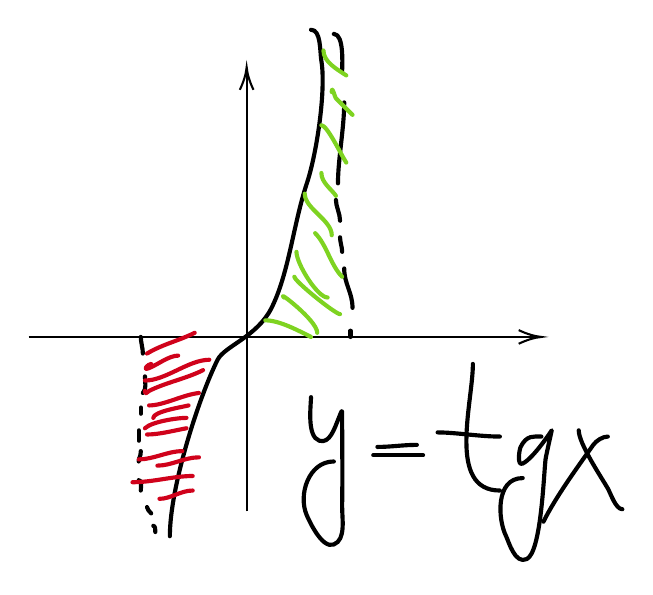
\begin{tikzpicture}[x=0.75pt,y=0.75pt,yscale=-1,xscale=1]
%uncomment if require: \path (0,412); %set diagram left start at 0, and has height of 412

%Straight Lines [id:da7309751331486005] 
\draw    (158,239) -- (403,239) ;
\draw [shift={(405,239)}, rotate = 180] [color={rgb, 255:red, 0; green, 0; blue, 0 }  ][line width=0.75]    (10.93,-3.29) .. controls (6.95,-1.4) and (3.31,-0.3) .. (0,0) .. controls (3.31,0.3) and (6.95,1.4) .. (10.93,3.29)   ;
%Straight Lines [id:da3867630169273685] 
\draw    (263,323) -- (263,111) ;
\draw [shift={(263,109)}, rotate = 90] [color={rgb, 255:red, 0; green, 0; blue, 0 }  ][line width=0.75]    (10.93,-3.29) .. controls (6.95,-1.4) and (3.31,-0.3) .. (0,0) .. controls (3.31,0.3) and (6.95,1.4) .. (10.93,3.29)   ;
%Shape: Free Drawing [id:dp0003972503350864187] 
\draw  [color={rgb, 255:red, 0; green, 0; blue, 0 }  ][line width=1.5] [line join = round][line cap = round] (226,335) .. controls (226,311.07) and (240.21,267.59) .. (249,250) .. controls (252.31,243.39) and (268.03,238.95) .. (275,225) .. controls (283.37,208.26) and (285.54,184.38) .. (292,165) .. controls (296.8,150.59) and (301.32,119.92) .. (299,106) .. controls (298.22,101.3) and (298.91,91) .. (294,91) ;
%Shape: Free Drawing [id:dp5201804636624221] 
\draw  [color={rgb, 255:red, 0; green, 0; blue, 0 }  ][line width=1.5] [line join = round][line cap = round] (212,239) .. controls (212,241.69) and (213,244.31) .. (213,247) ;
%Shape: Free Drawing [id:dp5851255907231582] 
\draw  [color={rgb, 255:red, 0; green, 0; blue, 0 }  ][line width=1.5] [line join = round][line cap = round] (214,258) .. controls (214,260.69) and (214.9,264.1) .. (213,266) ;
%Shape: Free Drawing [id:dp8815517761152026] 
\draw  [color={rgb, 255:red, 0; green, 0; blue, 0 }  ][line width=1.5] [line join = round][line cap = round] (212,273) .. controls (212,274) and (212,275) .. (212,276) ;
%Shape: Free Drawing [id:dp80520049266068] 
\draw  [color={rgb, 255:red, 0; green, 0; blue, 0 }  ][line width=1.5] [line join = round][line cap = round] (211,284) .. controls (211,285.67) and (211,287.33) .. (211,289) ;
%Shape: Free Drawing [id:dp316467359479106] 
\draw  [color={rgb, 255:red, 0; green, 0; blue, 0 }  ][line width=1.5] [line join = round][line cap = round] (212,294) .. controls (212,296.99) and (211,296.83) .. (211,299) ;
%Shape: Free Drawing [id:dp2834485693922434] 
\draw  [color={rgb, 255:red, 0; green, 0; blue, 0 }  ][line width=1.5] [line join = round][line cap = round] (211,308) .. controls (212.7,308) and (212,311.3) .. (212,313) ;
%Shape: Free Drawing [id:dp6159513818340512] 
\draw  [color={rgb, 255:red, 0; green, 0; blue, 0 }  ][line width=1.5] [line join = round][line cap = round] (215,321) .. controls (215,321.89) and (216.07,323.07) .. (217,324) ;
%Shape: Free Drawing [id:dp7891080275243103] 
\draw  [color={rgb, 255:red, 0; green, 0; blue, 0 }  ][line width=1.5] [line join = round][line cap = round] (218,330) .. controls (219.05,330) and (219,331.95) .. (219,333) ;
%Shape: Free Drawing [id:dp18224065945873258] 
\draw  [color={rgb, 255:red, 0; green, 0; blue, 0 }  ][line width=1.5] [line join = round][line cap = round] (305,93) .. controls (310.1,93) and (309,108.56) .. (309,111) ;
%Shape: Free Drawing [id:dp9620245827848797] 
\draw  [color={rgb, 255:red, 0; green, 0; blue, 0 }  ][line width=1.5] [line join = round][line cap = round] (310,126) .. controls (310,138.47) and (307,153.28) .. (307,165) ;
%Shape: Free Drawing [id:dp7133454851869357] 
\draw  [color={rgb, 255:red, 0; green, 0; blue, 0 }  ][line width=1.5] [line join = round][line cap = round] (306,173) .. controls (306,176.15) and (308,179.55) .. (308,183) ;
%Shape: Free Drawing [id:dp12386328513908185] 
\draw  [color={rgb, 255:red, 0; green, 0; blue, 0 }  ][line width=1.5] [line join = round][line cap = round] (308,191) .. controls (308,193.36) and (309,195.64) .. (309,198) ;
%Shape: Free Drawing [id:dp15587949383454502] 
\draw  [color={rgb, 255:red, 0; green, 0; blue, 0 }  ][line width=1.5] [line join = round][line cap = round] (310,206) .. controls (310,213.49) and (314,217.57) .. (314,225) ;
%Shape: Free Drawing [id:dp0761643181265077] 
\draw  [color={rgb, 255:red, 0; green, 0; blue, 0 }  ][line width=1.5] [line join = round][line cap = round] (313,236) .. controls (313,237) and (313,238) .. (313,239) ;
%Shape: Free Drawing [id:dp2021663107106323] 
\draw  [color={rgb, 255:red, 208; green, 2; blue, 27 }  ,draw opacity=1 ][line width=1.5] [line join = round][line cap = round] (215,247) .. controls (222.42,242.55) and (230.34,240.83) .. (238,237) ;
%Shape: Free Drawing [id:dp23152035679965066] 
\draw  [color={rgb, 255:red, 208; green, 2; blue, 27 }  ,draw opacity=1 ][line width=1.5] [line join = round][line cap = round] (217,252) .. controls (215.51,252) and (212.4,255.44) .. (216,254) .. controls (220.14,252.34) and (225.6,248) .. (230,248) ;
%Shape: Free Drawing [id:dp17795499674994364] 
\draw  [color={rgb, 255:red, 208; green, 2; blue, 27 }  ,draw opacity=1 ][line width=1.5] [line join = round][line cap = round] (214,260) .. controls (224.04,260) and (235,250) .. (245,250) ;
%Shape: Free Drawing [id:dp1865941792926743] 
\draw  [color={rgb, 255:red, 208; green, 2; blue, 27 }  ,draw opacity=1 ][line width=1.5] [line join = round][line cap = round] (214,265) .. controls (214,267.26) and (215.06,265.47) .. (216,265) .. controls (224.22,260.89) and (233.68,259.16) .. (242,255) ;
%Shape: Free Drawing [id:dp8778727815000686] 
\draw  [color={rgb, 255:red, 208; green, 2; blue, 27 }  ,draw opacity=1 ][line width=1.5] [line join = round][line cap = round] (216,272) .. controls (223.06,272) and (232.25,266.86) .. (240,266) ;
%Shape: Free Drawing [id:dp17239530417514104] 
\draw  [color={rgb, 255:red, 208; green, 2; blue, 27 }  ,draw opacity=1 ][line width=1.5] [line join = round][line cap = round] (218,278) .. controls (218,274.86) and (232.72,272.65) .. (235,272) ;
%Shape: Free Drawing [id:dp3456646149006728] 
\draw  [color={rgb, 255:red, 208; green, 2; blue, 27 }  ,draw opacity=1 ][line width=1.5] [line join = round][line cap = round] (214,283) .. controls (217.14,279.86) and (229.38,278) .. (234,278) ;
%Shape: Free Drawing [id:dp3339926968499365] 
\draw  [color={rgb, 255:red, 208; green, 2; blue, 27 }  ,draw opacity=1 ][line width=1.5] [line join = round][line cap = round] (211,298) .. controls (218.09,298) and (225.05,294) .. (232,294) ;
%Shape: Free Drawing [id:dp9522557706863325] 
\draw  [color={rgb, 255:red, 208; green, 2; blue, 27 }  ,draw opacity=1 ][line width=1.5] [line join = round][line cap = round] (220,301) .. controls (226.85,301) and (233.04,297) .. (240,297) ;
%Shape: Free Drawing [id:dp7452053877996763] 
\draw  [color={rgb, 255:red, 208; green, 2; blue, 27 }  ,draw opacity=1 ][line width=1.5] [line join = round][line cap = round] (208,309) .. controls (217.97,309) and (227.71,306) .. (237,306) ;
%Shape: Free Drawing [id:dp9823721194238563] 
\draw  [color={rgb, 255:red, 208; green, 2; blue, 27 }  ,draw opacity=1 ][line width=1.5] [line join = round][line cap = round] (221,317) .. controls (226.37,317) and (231.19,313) .. (237,313) ;
%Shape: Free Drawing [id:dp6933842797306785] 
\draw  [color={rgb, 255:red, 208; green, 2; blue, 27 }  ,draw opacity=1 ][line width=1.5] [line join = round][line cap = round] (215,286) .. controls (220.97,286) and (227.9,284.11) .. (234,283) ;
%Shape: Free Drawing [id:dp25553510430657356] 
\draw  [color={rgb, 255:red, 126; green, 211; blue, 33 }  ,draw opacity=1 ][line width=1.5] [line join = round][line cap = round] (272,231) .. controls (278.79,231) and (287.88,235.94) .. (294,239) ;
%Shape: Free Drawing [id:dp31019838318535986] 
\draw  [color={rgb, 255:red, 126; green, 211; blue, 33 }  ,draw opacity=1 ][line width=1.5] [line join = round][line cap = round] (281,220) .. controls (277.03,216.03) and (297,230.96) .. (297,237) ;
%Shape: Free Drawing [id:dp9076135131209477] 
\draw  [color={rgb, 255:red, 126; green, 211; blue, 33 }  ,draw opacity=1 ][line width=1.5] [line join = round][line cap = round] (286,210) .. controls (286,212.12) and (305.7,228) .. (308,228) ;
%Shape: Free Drawing [id:dp7971819088109766] 
\draw  [color={rgb, 255:red, 126; green, 211; blue, 33 }  ,draw opacity=1 ][line width=1.5] [line join = round][line cap = round] (287,198) .. controls (287,203.81) and (297.16,220) .. (302,220) ;
%Shape: Free Drawing [id:dp5319968818602678] 
\draw  [color={rgb, 255:red, 126; green, 211; blue, 33 }  ,draw opacity=1 ][line width=1.5] [line join = round][line cap = round] (296,189) .. controls (301.59,194.59) and (303.47,204.47) .. (309,210) ;
%Shape: Free Drawing [id:dp2660060573911053] 
\draw  [color={rgb, 255:red, 126; green, 211; blue, 33 }  ,draw opacity=1 ][line width=1.5] [line join = round][line cap = round] (291,170) .. controls (291,177.21) and (304,182.65) .. (304,190) ;
%Shape: Free Drawing [id:dp947217522533529] 
\draw  [color={rgb, 255:red, 126; green, 211; blue, 33 }  ,draw opacity=1 ][line width=1.5] [line join = round][line cap = round] (299,160) .. controls (299,164.66) and (303.83,167.74) .. (306,171) ;
%Shape: Free Drawing [id:dp8278283783958452] 
\draw  [color={rgb, 255:red, 126; green, 211; blue, 33 }  ,draw opacity=1 ][line width=1.5] [line join = round][line cap = round] (299,137) .. controls (301.82,137) and (308.36,151.04) .. (311,155) ;
%Shape: Free Drawing [id:dp4359165448328909] 
\draw  [color={rgb, 255:red, 126; green, 211; blue, 33 }  ,draw opacity=1 ][line width=1.5] [line join = round][line cap = round] (304,121) .. controls (304,117.44) and (305.56,123.56) .. (306,124) .. controls (308.54,126.54) and (311.17,129.17) .. (314,132) ;
%Shape: Free Drawing [id:dp7797802405551274] 
\draw  [color={rgb, 255:red, 126; green, 211; blue, 33 }  ,draw opacity=1 ][line width=1.5] [line join = round][line cap = round] (300,101) .. controls (300,106.54) and (306.74,110.16) .. (311,113) ;
%Shape: Free Drawing [id:dp7454151199683327] 
\draw  [color={rgb, 255:red, 0; green, 0; blue, 0 }  ,draw opacity=1 ][line width=1.5] [line join = round][line cap = round] (294,268) .. controls (294,271.89) and (291.85,286.95) .. (298,289) .. controls (303.1,290.7) and (305.49,282.53) .. (307,279) .. controls (307.59,277.63) and (309,273.51) .. (309,275) .. controls (309,290) and (309.25,305) .. (309,320) .. controls (308.89,326.47) and (311.01,336.6) .. (305,339) .. controls (299.18,341.33) and (292.8,326.8) .. (292,325) .. controls (287.62,315.15) and (292.84,299) .. (305,299) ;
%Shape: Free Drawing [id:dp8508397273539994] 
\draw  [color={rgb, 255:red, 0; green, 0; blue, 0 }  ,draw opacity=1 ][line width=1.5] [line join = round][line cap = round] (326,292) .. controls (332.34,292) and (338.66,291) .. (345,291) ;
%Shape: Free Drawing [id:dp4877929387816199] 
\draw  [color={rgb, 255:red, 0; green, 0; blue, 0 }  ,draw opacity=1 ][line width=1.5] [line join = round][line cap = round] (324,296) .. controls (332,296) and (340,296) .. (348,296) ;
%Shape: Free Drawing [id:dp9111208578093893] 
\draw  [color={rgb, 255:red, 0; green, 0; blue, 0 }  ,draw opacity=1 ][line width=1.5] [line join = round][line cap = round] (372,252) .. controls (372,270.58) and (359.31,313) .. (385,313) ;
%Shape: Free Drawing [id:dp7724522325014598] 
\draw  [color={rgb, 255:red, 0; green, 0; blue, 0 }  ,draw opacity=1 ][line width=1.5] [line join = round][line cap = round] (355,285) .. controls (363.77,285) and (375.17,287) .. (385,287) ;
%Shape: Free Drawing [id:dp6809009336292745] 
\draw  [color={rgb, 255:red, 0; green, 0; blue, 0 }  ,draw opacity=1 ][line width=1.5] [line join = round][line cap = round] (405,287) .. controls (401.28,287) and (397.93,286.14) .. (395,292) .. controls (394.33,293.35) and (393.14,301.43) .. (396,300) .. controls (401.25,297.37) and (410,284) .. (410,284) .. controls (410,284) and (407.16,296.58) .. (407,298) .. controls (406.08,306.27) and (404.85,342.58) .. (398,346) .. controls (392.28,348.86) and (389.21,337.42) .. (388,335) .. controls (383.92,326.83) and (382.85,307) .. (396,307) ;
%Shape: Free Drawing [id:dp8276969647642894] 
\draw  [color={rgb, 255:red, 0; green, 0; blue, 0 }  ,draw opacity=1 ][line width=1.5] [line join = round][line cap = round] (423,284) .. controls (423,290.39) and (433.98,306.72) .. (437,312) .. controls (438.47,314.58) and (440.81,322) .. (444,322) ;
%Shape: Free Drawing [id:dp598325833870565] 
\draw  [color={rgb, 255:red, 0; green, 0; blue, 0 }  ,draw opacity=1 ][line width=1.5] [line join = round][line cap = round] (437,287) .. controls (434.57,287) and (431.47,288.92) .. (430,291) .. controls (422.11,302.18) and (412.07,315.85) .. (406,328) ;




\end{tikzpicture}



В таком случае заводят интерграл в смысле главного значения

$v.p. \int_{\pi / 2}^{\pi / 2} tgx dx = \lim_{B\to \pi / 2} \int_{-B}^B = 0$

По аналогии $v.p. \int_{-1}^1 \frac{1}{x} = 0$, но при этом первообрзная $\log$

$\but$ в $v.p. $ нельзя делать замену переменной, т.к. предполагается, что окресность симметричная

\item \[
    \int_{10}^{\infty} x^\al (\log x) ^ \be \text{ основная идея 'удавливание логарифма'}
    \]

\begin{enumerate}
    \item  $\al < -1, \al = -1 - \varepsilon, x ^ \al (\log x) ^\be = x ^ {-1 - \varepsilon / 2} \cdot \underbrace{x ^ {-\varepsilon / 2} (\log x) ^ \be}_{\text{огр. на $[10, +\infty)$}} \leqslant C \cdot x ^ {-1 - \varepsilon / 2} \hence \text{сходится}$
    
    \item $\al > -1, \al = -1 + \varepsilon, x ^ \al (\log x) ^\be = x ^ {-1 + \varepsilon / 2} \cdot \underbrace{x ^ {\varepsilon / 2} (\log x) ^ {\be}}_{\to \infty, x \to \infty} \geqslant C \cdot x ^ {-1 + \varepsilon / 2} \hence \text{расходится}$
    
    \item $\al = -1, \int_{10}^{\infty} \frac{(\log x) ^ \be}{x} dx = \int_{10}^{\infty} (\log x) ^ \be d(\log x) \hence \text{сх-ся $\Longleftrightarrow \be < -1 $ }$
\end{enumerate}
\end{enumerate} 
\end{examples}


\quad

$\int_0^\infty \frac{sinx}{x} dx$ сходится ли?

    

\tikzset{every picture/.style={line width=0.75pt}} %set default line width to 0.75pt        

\begin{tikzpicture}[x=0.75pt,y=0.75pt,yscale=-1,xscale=1]
%uncomment if require: \path (0,412); %set diagram left start at 0, and has height of 412

%Straight Lines [id:da45685719020165094] 
\draw    (135,229) -- (477,229) ;
\draw [shift={(479,229)}, rotate = 180] [color={rgb, 255:red, 0; green, 0; blue, 0 }  ][line width=0.75]    (10.93,-3.29) .. controls (6.95,-1.4) and (3.31,-0.3) .. (0,0) .. controls (3.31,0.3) and (6.95,1.4) .. (10.93,3.29)   ;
%Straight Lines [id:da6318090955802496] 
\draw    (259,337) -- (259,63) ;
\draw [shift={(259,61)}, rotate = 90] [color={rgb, 255:red, 0; green, 0; blue, 0 }  ][line width=0.75]    (10.93,-3.29) .. controls (6.95,-1.4) and (3.31,-0.3) .. (0,0) .. controls (3.31,0.3) and (6.95,1.4) .. (10.93,3.29)   ;
%Shape: Free Drawing [id:dp38358030787495656] 
\draw  [color={rgb, 255:red, 0; green, 0; blue, 0 }  ,draw opacity=1 ][line width=1.5] [line join = round][line cap = round] (258,180) .. controls (265.01,180) and (272.73,177.87) .. (279,181) .. controls (289.22,186.11) and (298.74,211.46) .. (301,225) .. controls (303.22,238.34) and (303.18,259.73) .. (316,264) .. controls (320.77,265.59) and (328.35,258.44) .. (332,256) .. controls (349.05,244.63) and (346.68,210.89) .. (364,208) .. controls (379.36,205.44) and (386.05,222.05) .. (393,229) .. controls (396.57,232.57) and (397.43,239.91) .. (404,241) .. controls (410.32,242.05) and (417.73,235.8) .. (419,232) .. controls (420.18,228.45) and (421.52,220.44) .. (425,220) .. controls (446.51,217.31) and (439.82,238.27) .. (451,242) .. controls (459.85,244.95) and (458.48,228.22) .. (459,223) .. controls (459.07,222.26) and (459.26,221.09) .. (460,221) .. controls (469.61,219.8) and (471.2,224) .. (474,231) .. controls (475.23,234.08) and (478,235.8) .. (478,238) ;




\end{tikzpicture}


\begin{namedtheorem}{признаки Дирихле и Абеля}
    $f, g \in C[a, b], g \in C^1[a, b], \int_a^{\to b} fg dx$
\end{namedtheorem}

\begin{namedtheorem}{признак Дирихле}
    $F $ --- первообразная f, F --- огр., g --- монотон., $g \to 0$ при $x \to b- \hence \int_a^{\to b} fg dx $ сх-ся
\end{namedtheorem}


\begin{namedtheorem}{признак Абеля}
    $\underbrace{\int_a^{\to b} f dx}_{\Leftrightarrow \exists \lim_{x \to b-} F(x)}$ сходится, $g$ --- монот. и огр. $\hence \int_a^{\to b} fg dx $ сх-ся
\end{namedtheorem}


\begin{proof}
    \[
        \int_a^B fg dx = \int_a^B g dF = Fg \bigg| _a ^ B - \int_a^B F g' dx 
    \]

    Хотим устремить $B \to b-$
    
    Посмотрим на двойную подстановку
    
    (п.Д.) $F$ --- ограничено в $b-$, $g(x) \to 0 \hence F(x)g(x) \to 0, $ при $x \to b-$

    (п.А.) $F$ имеет предел, $g(x)$ тоже имеет предел $\exists \lim_{x \to b-} F, \lim_{x  \to b-} g \hence \exists \lim_{x\to b-} Fg$

    Следовательно, и в признаке Дирихле и в признаке Абеля двоя подстановка определена

    Теперь посмотрим на $\int_a^B Fg' dx$.

    (п.Д.) $\int_a^B \abs{Fg'} dx$, $g'$ не меняет знак, $F$ ограничена.

    \[
        \int_a^B \abs{Fg'} dx \leqslant \sup \abs{F} \int_a^B \abs{g'} dx = \int_a^B \abs{Fg'} dx \leqslant \sup \abs{F} \cdot \abs{g(B) - g(a)} \to \sup \abs{F} \cdot \abs{0 - g(a)}
    \]

    $\hence $ есть абсолютная сходимость $\int_a^B Fg' dx$

    (п.А.) $\int_a^B \abs{Fg'} dx$, $g'$ не меняет знак, $F$ ограничена.


    \[
        \int_a^B \abs{Fg'} dx \leqslant \sup \abs{F} \int_a^B \abs{g'} dx = \int_a^B \abs{Fg'} dx \leqslant \sup \abs{F} \cdot \abs{g(B) - g(a)} \to \sup \abs{F} \cdot \abs{g(b-) - g(a)}
    \]

\end{proof}


\begin{examples}
\begin{enumerate}
    \item \[
        \int_{10}^{+\infty} \frac{\sin x}{x ^ \alpha} dx
    \]

    \begin{remark}
        $
        \begin{cases}
            \alpha > 1 \hence  \text{ абсолютная сходимость} \\
            \alpha \in (0, 1) \hence \text{ условная сходимость } \int_{10}^{+\infty} \frac{\abs{\sin x}}{x ^ \alpha} dx \geqslant \int_{10}^{+\infty} \frac{\sin ^ 2 x}{x ^ \alpha} dx = \underbrace{\int_{10}^{+\infty} \frac{1 - \cos 2x}{2 x ^ \alpha} dx}_{\text{расх. + сх.}}
        \end{cases}
        $
    \end{remark}
    

$\left. 
    \begin{array}{lr}
    \sin x \text{ имеет ограниченную первообрзную} \\
    \alpha > 0 \hence \frac{1}{x ^ \alpha} \dec 0
    \end{array}
 \right\} \hence \alpha > 0 \hence $ интерграл сходится

\quad

$\but$ не стоит думать про интергралы, как про ряды. Контрпример:

$\int_{10}^{+\infty} \sin(x^2) dx = C \cdot \int_{?}^{+\infty} \frac{\sin y}{\sqrt{y}} dy$ и т.к. $\alpha > 0$ он сходится, хотя общий член к нулю не стремится.


\quad

$\al \geqslant 0$ --- Критерий Коши

\quad 

\quad

    \item $\int_{10}^{\infty} \underbrace{\frac{\sin x}{x ^ \alpha}}_{f} \cdot \underbrace{\arctan \sqrt{x}}_{g}$. Заметим, что $\int f$ сходится, а $g$ --- монотонна и ограничена $\hence$ по признаку Абеля сходится.
\end{enumerate}
    

\end{examples}


\subsection{Вычисление площадей и объемов}

\begin{enumerate}
    \item $f \in C[a, b], f \geqslant 0 S(P_f[a, b]) = \int_a^b f dx$ --- площадь подграфика.
    \item Площадь криволинейной трапеции
    
    $f, g \in C[a, b], f \geqslant g \hence S(\Phi) = \int_a^b (f - g) dx$

    \tikzset{every picture/.style={line width=0.75pt}} %set default line width to 0.75pt        
    
    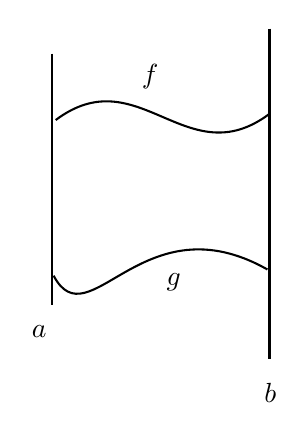
\begin{tikzpicture}[x=0.75pt,y=0.75pt,yscale=-1,xscale=1]
    %uncomment if require: \path (0,412); %set diagram left start at 0, and has height of 412
    
    %Straight Lines [id:da820525410689766] 
    \draw    (100,119) -- (100,240) ;
    %Straight Lines [id:da45348289406040343] 
    \draw    (205,107) -- (205,266) ;
    %Curve Lines [id:da3017264890378202] 
    \draw    (102,151) .. controls (142,121) and (165,178) .. (205,148) ;
    %Curve Lines [id:da09887112140791576] 
    \draw    (101,226) .. controls (118,258) and (144,189) .. (204,223) ;
    
    % Text Node
    \draw (142,122.4) node [anchor=north west][inner sep=0.75pt]    {$f$};
    % Text Node
    \draw (154,223.4) node [anchor=north west][inner sep=0.75pt]    {$g$};
    % Text Node
    \draw (89,248.4) node [anchor=north west][inner sep=0.75pt]    {$a$};
    % Text Node
    \draw (201,276.4) node [anchor=north west][inner sep=0.75pt]    {$b$};
    
    
    \end{tikzpicture}
    
    
    \item $f : [\alpha, \be] \to \R_+ = [0, +\infty)$, $0 \leqslant \al < \be \leqslant 2 \pi $, $\{ (r, \phi) | \phi \in [\al, \be], r \in [0, f(\phi)] \} = \widetilde{P}_f$ --- криволинейный сектор, $f \in C[\al, \be]$
   

\tikzset{every picture/.style={line width=0.75pt}} %set default line width to 0.75pt        

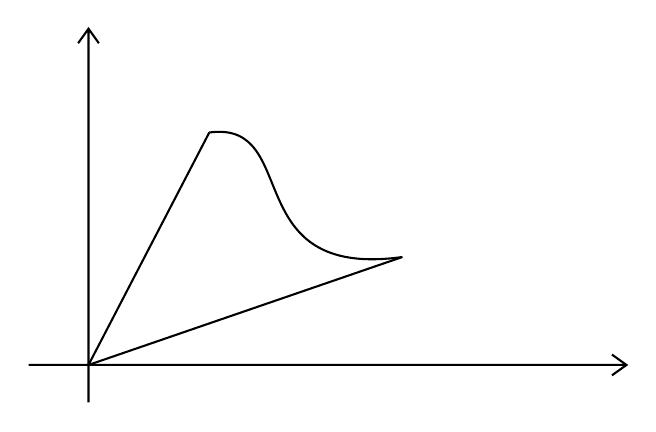
\begin{tikzpicture}[x=0.75pt,y=0.75pt,yscale=-1,xscale=1]
%uncomment if require: \path (0,412); %set diagram left start at 0, and has height of 412

%Shape: Axis 2D [id:dp6700788822304291] 
\draw  (176,257) -- (464,257)(204.8,95) -- (204.8,275) (457,252) -- (464,257) -- (457,262) (199.8,102) -- (204.8,95) -- (209.8,102)  ;
%Straight Lines [id:da06852563223272257] 
\draw    (356,205) -- (204.8,257) ;
%Straight Lines [id:da9246611817647475] 
\draw    (263,145) -- (204.8,257) ;
%Curve Lines [id:da6989609572657072] 
\draw    (263,145) .. controls (308,139) and (276,216) .. (356,205) ;




\end{tikzpicture}



$S(\widetilde{P}_f) = \frac{1}{2} \int_\al^\be (f(\phi))^2 d\phi$

\begin{enumerate}
    \item Уверуем в площадь сектора
    



    \tikzset{every picture/.style={line width=0.75pt}} %set default line width to 0.75pt        

    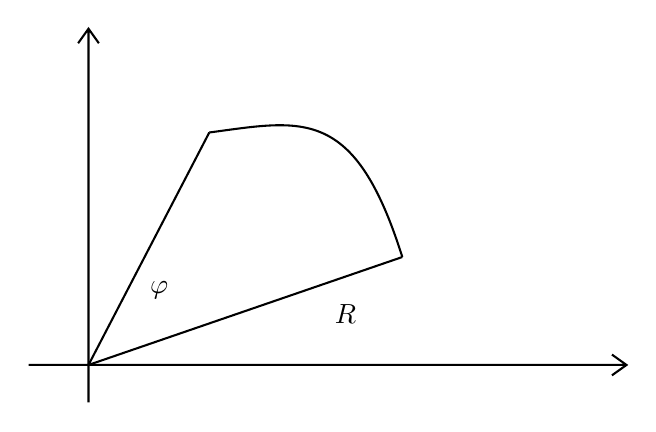
\begin{tikzpicture}[x=0.75pt,y=0.75pt,yscale=-1,xscale=1]
    %uncomment if require: \path (0,412); %set diagram left start at 0, and has height of 412
    
    %Shape: Axis 2D [id:dp6700788822304291] 
    \draw  (176,257) -- (464,257)(204.8,95) -- (204.8,275) (457,252) -- (464,257) -- (457,262) (199.8,102) -- (204.8,95) -- (209.8,102)  ;
    %Straight Lines [id:da06852563223272257] 
    \draw    (356,205) -- (204.8,257) ;
    %Straight Lines [id:da9246611817647475] 
    \draw    (263,145) -- (204.8,257) ;
    %Curve Lines [id:da6989609572657072] 
    \draw    (263,145) .. controls (308,139) and (333,132) .. (356,205) ;
    
    % Text Node
    \draw (233,215.4) node [anchor=north west][inner sep=0.75pt]    {$\varphi $};
    % Text Node
    \draw (322,226.4) node [anchor=north west][inner sep=0.75pt]    {$R$};
    
    
    \end{tikzpicture}
    
    $S = \frac{\phi}{2 \pi} \pi R^2 =  \frac{\phi}{2} R^2$


    \item Строим дробление

    \tikzset{every picture/.style={line width=0.75pt}} %set default line width to 0.75pt        
    
    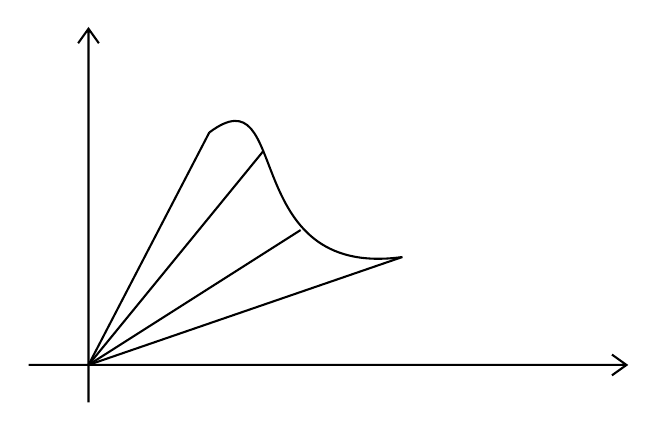
\begin{tikzpicture}[x=0.75pt,y=0.75pt,yscale=-1,xscale=1]
    %uncomment if require: \path (0,412); %set diagram left start at 0, and has height of 412
    
    %Shape: Axis 2D [id:dp6700788822304291] 
    \draw  (176,257) -- (464,257)(204.8,95) -- (204.8,275) (457,252) -- (464,257) -- (457,262) (199.8,102) -- (204.8,95) -- (209.8,102)  ;
    %Straight Lines [id:da06852563223272257] 
    \draw    (356,205) -- (204.8,257) ;
    %Straight Lines [id:da9246611817647475] 
    \draw    (263,145) -- (204.8,257) ;
    %Curve Lines [id:da6989609572657072] 
    \draw    (263,145) .. controls (303,115) and (276,216) .. (356,205) ;
    %Straight Lines [id:da8056749445450382] 
    \draw    (289,154) -- (204.8,257) ;
    %Straight Lines [id:da9648917490356489] 
    \draw    (307,192) -- (204.8,257) ;
    
    
    
    
    \end{tikzpicture}
    
    $\alpha = \phi_0 < \phi_1 < ... < \phi_n = \be$

    

\tikzset{every picture/.style={line width=0.75pt}} %set default line width to 0.75pt        

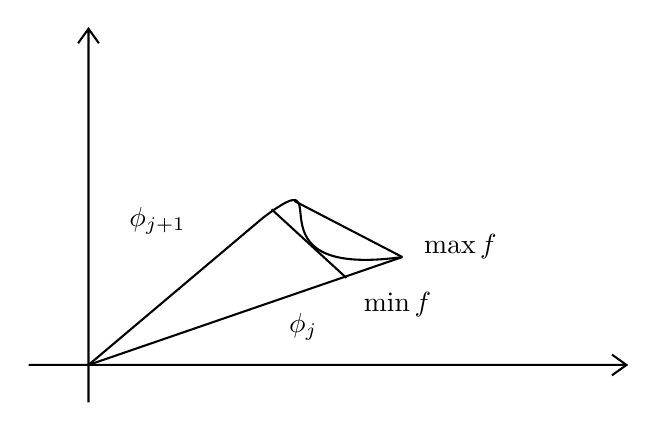
\begin{tikzpicture}[x=0.75pt,y=0.75pt,yscale=-1,xscale=1]
%uncomment if require: \path (0,412); %set diagram left start at 0, and has height of 412

%Shape: Axis 2D [id:dp6700788822304291] 
\draw  (176,257) -- (464,257)(204.8,95) -- (204.8,275) (457,252) -- (464,257) -- (457,262) (199.8,102) -- (204.8,95) -- (209.8,102)  ;
%Straight Lines [id:da06852563223272257] 
\draw    (356,205) -- (204.8,257) ;
%Straight Lines [id:da9246611817647475] 
\draw    (289,186) -- (204.8,257) ;
%Curve Lines [id:da6989609572657072] 
\draw    (289,186) .. controls (329,156) and (276,216) .. (356,205) ;
%Straight Lines [id:da8968556069693085] 
\draw    (293,182) -- (329,215) ;
%Straight Lines [id:da37934960247256855] 
\draw    (304,178) -- (356,205) ;

% Text Node
\draw (223,179.4) node [anchor=north west][inner sep=0.75pt]    {$\phi _{j+1}$};
% Text Node
\draw (300,230.4) node [anchor=north west][inner sep=0.75pt]    {$\phi _{j}$};
% Text Node
\draw (365,192.4) node [anchor=north west][inner sep=0.75pt]    {$\max f$};
% Text Node
\draw (336,220.4) node [anchor=north west][inner sep=0.75pt]    {$\min f$};


\end{tikzpicture}

\[
    \underbrace{\sum_{j=1}^n \frac{(\min_{\phi_{j-1},\phi_j} f) ^ 2 (\phi_j - \phi_{j - 1})}{2} \leqslant S(\widetilde{P}_f) \leqslant \sum_{j=1}^n \frac{(\max_{\phi_{j-1},\phi_j} f) ^ 2 (\phi_j - \phi_{j - 1})}{2}}_{\to \frac{1}{2} \int_\al^\be f^2 d\phi}
\]

\end{enumerate}

\newpage

\item $\gamma(t) = (x(t), y(t)), t \in [a, b]$



\tikzset{every picture/.style={line width=0.75pt}} %set default line width to 0.75pt        

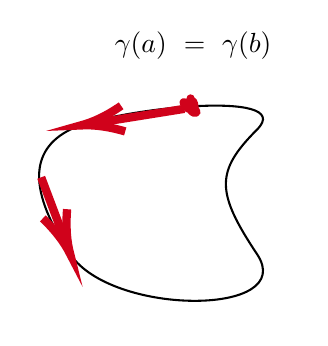
\begin{tikzpicture}[x=0.75pt,y=0.75pt,yscale=-1,xscale=1]
%uncomment if require: \path (0,412); %set diagram left start at 0, and has height of 412

%Shape: Polygon Curved [id:ds7942562138886865] 
\draw   (226,203) .. controls (246,193) and (336,183) .. (316,203) .. controls (296,223) and (296,233) .. (316,263) .. controls (336,293) and (246,293) .. (226,263) .. controls (206,233) and (206,213) .. (226,203) -- cycle ;
%Straight Lines [id:da8426195840306461] 
\draw [color={rgb, 255:red, 208; green, 2; blue, 27 }  ,draw opacity=1 ][line width=3]    (281,193) -- (235.94,200.21) ;
\draw [shift={(231,201)}, rotate = 350.91] [color={rgb, 255:red, 208; green, 2; blue, 27 }  ,draw opacity=1 ][line width=3]    (20.77,-6.25) .. controls (13.2,-2.65) and (6.28,-0.57) .. (0,0) .. controls (6.28,0.57) and (13.2,2.66) .. (20.77,6.25)   ;
%Straight Lines [id:da9344582541710046] 
\draw [color={rgb, 255:red, 208; green, 2; blue, 27 }  ,draw opacity=1 ][line width=3]    (212,226) -- (224.23,258.32) ;
\draw [shift={(226,263)}, rotate = 249.27] [color={rgb, 255:red, 208; green, 2; blue, 27 }  ,draw opacity=1 ][line width=3]    (20.77,-6.25) .. controls (13.2,-2.65) and (6.28,-0.57) .. (0,0) .. controls (6.28,0.57) and (13.2,2.66) .. (20.77,6.25)   ;
%Shape: Free Drawing [id:dp40068082619101875] 
\draw  [color={rgb, 255:red, 208; green, 2; blue, 27 }  ,draw opacity=1 ][line width=3] [line join = round][line cap = round] (283,193) .. controls (274.91,184.91) and (290.41,195) .. (286,195) .. controls (283.89,195) and (282.11,189.94) .. (284,189) .. controls (285.61,188.2) and (286,192.2) .. (286,194) .. controls (286,196.11) and (284,190.11) .. (284,188) ;

% Text Node
\draw (246,154.4) node [anchor=north west][inner sep=0.75pt]    {$\gamma ( a) \ =\ \gamma ( b)$};


\end{tikzpicture}

Хотим считать площадь

\quad

% Pattern Info
 
\tikzset{
pattern size/.store in=\mcSize, 
pattern size = 5pt,
pattern thickness/.store in=\mcThickness, 
pattern thickness = 0.3pt,
pattern radius/.store in=\mcRadius, 
pattern radius = 1pt}
\makeatletter
\pgfutil@ifundefined{pgf@pattern@name@_mkpgbwn5v}{
\pgfdeclarepatternformonly[\mcThickness,\mcSize]{_mkpgbwn5v}
{\pgfqpoint{0pt}{-\mcThickness}}
{\pgfpoint{\mcSize}{\mcSize}}
{\pgfpoint{\mcSize}{\mcSize}}
{
\pgfsetcolor{\tikz@pattern@color}
\pgfsetlinewidth{\mcThickness}
\pgfpathmoveto{\pgfqpoint{0pt}{\mcSize}}
\pgfpathlineto{\pgfpoint{\mcSize+\mcThickness}{-\mcThickness}}
\pgfusepath{stroke}
}}
\makeatother
\tikzset{every picture/.style={line width=0.75pt}} %set default line width to 0.75pt        

\begin{tikzpicture}[x=0.75pt,y=0.75pt,yscale=-1,xscale=1]
%uncomment if require: \path (0,412); %set diagram left start at 0, and has height of 412

%Shape: Circle [id:dp3489340786869164] 
\draw  [pattern=_mkpgbwn5v,pattern size=6pt,pattern thickness=0.75pt,pattern radius=0pt, pattern color={rgb, 255:red, 208; green, 2; blue, 27}] (225,210) .. controls (225,179.07) and (250.07,154) .. (281,154) .. controls (311.93,154) and (337,179.07) .. (337,210) .. controls (337,240.93) and (311.93,266) .. (281,266) .. controls (250.07,266) and (225,240.93) .. (225,210) -- cycle ;

% Text Node
\draw (237,122.4) node [anchor=north west][inner sep=0.75pt]    {$(\cos t,\ \sin \ t)$};


\end{tikzpicture}

Плохая ситуация, т.к. нельзя провести две вертикальные прямые и посчтать как площадь криволинейной трапеции, но можно разбить на много параметрически заданных криволинейных трапеций:



\tikzset{every picture/.style={line width=0.75pt}} %set default line width to 0.75pt        

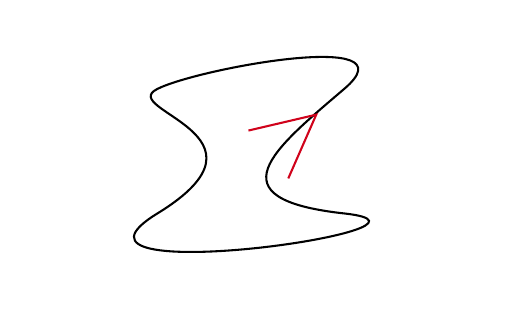
\begin{tikzpicture}[x=0.75pt,y=0.75pt,yscale=-1,xscale=1]
%uncomment if require: \path (0,412); %set diagram left start at 0, and has height of 412

%Shape: Polygon Curved [id:ds4998966965524809] 
\draw   (227,208) .. controls (247,198) and (351,179) .. (317,208) .. controls (283,237) and (253,261) .. (317,268) .. controls (381,275) and (165,306) .. (227,268) .. controls (289,230) and (207,218) .. (227,208) -- cycle ;
\draw  [color={rgb, 255:red, 208; green, 2; blue, 27 }  ,draw opacity=1 ] (270.88,228.06) -- (303.53,220.41) -- (290.06,251.12) ;




\end{tikzpicture}
 
\newpage




\tikzset{every picture/.style={line width=0.75pt}} %set default line width to 0.75pt        

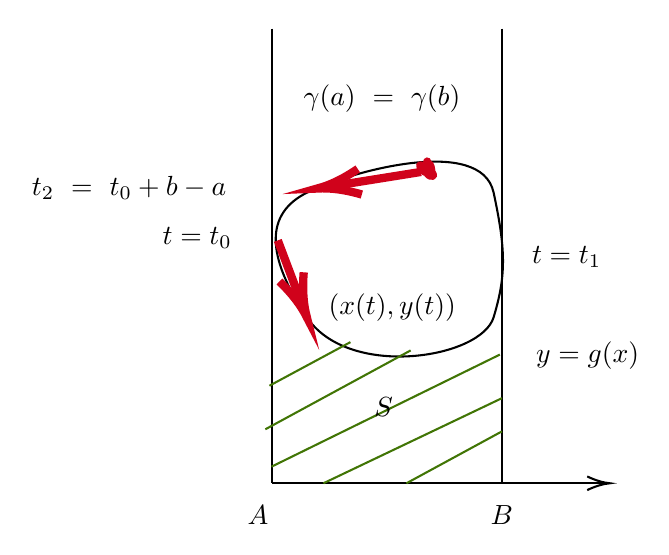
\begin{tikzpicture}[x=0.75pt,y=0.75pt,yscale=-1,xscale=1]
%uncomment if require: \path (0,412); %set diagram left start at 0, and has height of 412

%Shape: Polygon Curved [id:ds7942562138886865] 
\draw   (226,203) .. controls (246,193) and (310,175) .. (316,203) .. controls (322,231) and (322,243) .. (316,263) .. controls (310,283) and (246,293) .. (226,263) .. controls (206,233) and (206,213) .. (226,203) -- cycle ;
%Straight Lines [id:da8426195840306461] 
\draw [color={rgb, 255:red, 208; green, 2; blue, 27 }  ,draw opacity=1 ][line width=3]    (281,193) -- (235.94,200.21) ;
\draw [shift={(231,201)}, rotate = 350.91] [color={rgb, 255:red, 208; green, 2; blue, 27 }  ,draw opacity=1 ][line width=3]    (20.77,-6.25) .. controls (13.2,-2.65) and (6.28,-0.57) .. (0,0) .. controls (6.28,0.57) and (13.2,2.66) .. (20.77,6.25)   ;
%Straight Lines [id:da9344582541710046] 
\draw [color={rgb, 255:red, 208; green, 2; blue, 27 }  ,draw opacity=1 ][line width=3]    (212,226) -- (224.23,258.32) ;
\draw [shift={(226,263)}, rotate = 249.27] [color={rgb, 255:red, 208; green, 2; blue, 27 }  ,draw opacity=1 ][line width=3]    (20.77,-6.25) .. controls (13.2,-2.65) and (6.28,-0.57) .. (0,0) .. controls (6.28,0.57) and (13.2,2.66) .. (20.77,6.25)   ;
%Shape: Free Drawing [id:dp40068082619101875] 
\draw  [color={rgb, 255:red, 208; green, 2; blue, 27 }  ,draw opacity=1 ][line width=3] [line join = round][line cap = round] (283,193) .. controls (274.91,184.91) and (290.41,195) .. (286,195) .. controls (283.89,195) and (282.11,189.94) .. (284,189) .. controls (285.61,188.2) and (286,192.2) .. (286,194) .. controls (286,196.11) and (284,190.11) .. (284,188) ;
%Straight Lines [id:da8653614779259214] 
\draw    (209,124) -- (209,343) ;
%Straight Lines [id:da9114230868492257] 
\draw    (320,124) -- (320,343) ;
%Straight Lines [id:da03052310868084973] 
\draw    (209,343) -- (370,343) ;
\draw [shift={(372,343)}, rotate = 180] [color={rgb, 255:red, 0; green, 0; blue, 0 }  ][line width=0.75]    (10.93,-3.29) .. controls (6.95,-1.4) and (3.31,-0.3) .. (0,0) .. controls (3.31,0.3) and (6.95,1.4) .. (10.93,3.29)   ;
%Straight Lines [id:da026630072882267708] 
\draw [color={rgb, 255:red, 65; green, 117; blue, 5 }  ,draw opacity=1 ]   (319,281) -- (209,335) ;
%Straight Lines [id:da462598972817152] 
\draw [color={rgb, 255:red, 65; green, 117; blue, 5 }  ,draw opacity=1 ]   (320,302) -- (234,343) ;
%Straight Lines [id:da5601832084595084] 
\draw [color={rgb, 255:red, 65; green, 117; blue, 5 }  ,draw opacity=1 ]   (320,318) -- (274,343) ;
%Straight Lines [id:da1951888009445505] 
\draw [color={rgb, 255:red, 65; green, 117; blue, 5 }  ,draw opacity=1 ]   (276,279) -- (206,317) ;
%Straight Lines [id:da8578706741933491] 
\draw [color={rgb, 255:red, 65; green, 117; blue, 5 }  ,draw opacity=1 ]   (247,275) -- (208,296) ;

% Text Node
\draw (223,149.4) node [anchor=north west][inner sep=0.75pt]    {$\gamma ( a) \ =\ \gamma ( b)$};
% Text Node
\draw (155,218.4) node [anchor=north west][inner sep=0.75pt]    {$t=t_{0}$};
% Text Node
\draw (333,227.4) node [anchor=north west][inner sep=0.75pt]    {$t=t_{1}$};
% Text Node
\draw (257,300.4) node [anchor=north west][inner sep=0.75pt]    {$S$};
% Text Node
\draw (235,250.4) node [anchor=north west][inner sep=0.75pt]    {$( x( t) ,y( t))$};
% Text Node
\draw (196,352.4) node [anchor=north west][inner sep=0.75pt]    {$A$};
% Text Node
\draw (313,352.4) node [anchor=north west][inner sep=0.75pt]    {$B$};
% Text Node
\draw (335,273.4) node [anchor=north west][inner sep=0.75pt]    {$y=g( x)$};
% Text Node
\draw (92,193.4) node [anchor=north west][inner sep=0.75pt]    {$t_{2} \ =\ t_{0} +b-a$};


\end{tikzpicture}



$S_{\text{нижн.}} = \int_A^B g(x) dx = \int_{t_0}^{t_1} y(x(t)) x'(t) dt$ (сделали замену переменной) $ = \int_{t_0}^{t_1} y(t) x'(t) dt$

$S_{\text{верх.}} = -\int_{t_1}^{t_2} y(t) x'(t) dt$

$S = - \int_a^b y(t) x'(t) dt = - xy \bigg |_a ^ b + \int_a^b y'(t) x(t) dt $

$\but$ На восьмерке сломается, т.к. есть самопересечения



\tikzset{every picture/.style={line width=0.75pt}} %set default line width to 0.75pt        

\begin{tikzpicture}[x=0.75pt,y=0.75pt,yscale=-1,xscale=1]
%uncomment if require: \path (0,412); %set diagram left start at 0, and has height of 412

%Shape: Polygon Curved [id:ds8511771897060294] 
\draw   (219,205) .. controls (235,223) and (293,161) .. (336,198) .. controls (379,235) and (311,259) .. (284,247) .. controls (257,235) and (259,190) .. (246,158) .. controls (233,126) and (217,135) .. (194,151) .. controls (171,167) and (203,187) .. (219,205) -- cycle ;




\end{tikzpicture}

\item Вычисление объемов


\tikzset{every picture/.style={line width=0.75pt}} %set default line width to 0.75pt        

\begin{tikzpicture}[x=0.75pt,y=0.75pt,yscale=-1,xscale=1]
%uncomment if require: \path (0,412); %set diagram left start at 0, and has height of 412

%Shape: Polygon Curved [id:ds685815905131548] 
\draw   (186,164) .. controls (207,172) and (240,136) .. (276,164) .. controls (312,192) and (344,199) .. (276,224) .. controls (208,249) and (212,243) .. (186,224) .. controls (160,205) and (165,156) .. (186,164) -- cycle ;
%Shape: Arc [id:dp2731985158344479] 
\draw  [draw opacity=0][dash pattern={on 0.84pt off 2.51pt}] (187.5,224.48) .. controls (181.03,219.51) and (176.54,208.53) .. (176.54,195.78) .. controls (176.54,178.36) and (184.92,164.24) .. (195.27,164.24) .. controls (196.25,164.24) and (197.21,164.36) .. (198.15,164.61) -- (195.27,195.78) -- cycle ; \draw  [dash pattern={on 0.84pt off 2.51pt}] (187.5,224.48) .. controls (181.03,219.51) and (176.54,208.53) .. (176.54,195.78) .. controls (176.54,178.36) and (184.92,164.24) .. (195.27,164.24) .. controls (196.25,164.24) and (197.21,164.36) .. (198.15,164.61) ;  
%Shape: Arc [id:dp0786092918848319] 
\draw  [draw opacity=0][dash pattern={on 0.84pt off 2.51pt}] (192.01,226.9) .. controls (192.54,227.17) and (193.08,227.31) .. (193.64,227.31) .. controls (199.23,227.31) and (203.77,213.19) .. (203.77,195.78) .. controls (203.77,178.36) and (199.23,164.24) .. (193.64,164.24) .. controls (192.67,164.24) and (191.73,164.66) .. (190.84,165.46) -- (193.64,195.78) -- cycle ; \draw  [dash pattern={on 0.84pt off 2.51pt}] (192.01,226.9) .. controls (192.54,227.17) and (193.08,227.31) .. (193.64,227.31) .. controls (199.23,227.31) and (203.77,213.19) .. (203.77,195.78) .. controls (203.77,178.36) and (199.23,164.24) .. (193.64,164.24) .. controls (192.67,164.24) and (191.73,164.66) .. (190.84,165.46) ;  
%Shape: Arc [id:dp2439339338907578] 
\draw  [draw opacity=0][dash pattern={on 0.84pt off 2.51pt}] (264.5,222.48) .. controls (258.03,217.51) and (253.54,206.53) .. (253.54,193.78) .. controls (253.54,176.36) and (261.92,162.24) .. (272.27,162.24) .. controls (273.25,162.24) and (274.21,162.36) .. (275.15,162.61) -- (272.27,193.78) -- cycle ; \draw  [dash pattern={on 0.84pt off 2.51pt}] (264.5,222.48) .. controls (258.03,217.51) and (253.54,206.53) .. (253.54,193.78) .. controls (253.54,176.36) and (261.92,162.24) .. (272.27,162.24) .. controls (273.25,162.24) and (274.21,162.36) .. (275.15,162.61) ;  
%Shape: Arc [id:dp245133205800679] 
\draw  [draw opacity=0][dash pattern={on 0.84pt off 2.51pt}] (269.01,224.9) .. controls (269.54,225.17) and (270.08,225.31) .. (270.64,225.31) .. controls (276.23,225.31) and (280.77,211.19) .. (280.77,193.78) .. controls (280.77,176.36) and (276.23,162.24) .. (270.64,162.24) .. controls (269.67,162.24) and (268.73,162.66) .. (267.84,163.46) -- (270.64,193.78) -- cycle ; \draw  [dash pattern={on 0.84pt off 2.51pt}] (269.01,224.9) .. controls (269.54,225.17) and (270.08,225.31) .. (270.64,225.31) .. controls (276.23,225.31) and (280.77,211.19) .. (280.77,193.78) .. controls (280.77,176.36) and (276.23,162.24) .. (270.64,162.24) .. controls (269.67,162.24) and (268.73,162.66) .. (267.84,163.46) ;  
%Straight Lines [id:da28757468739997916] 
\draw    (138,281) -- (350,281) ;
\draw [shift={(352,281)}, rotate = 180] [color={rgb, 255:red, 0; green, 0; blue, 0 }  ][line width=0.75]    (10.93,-3.29) .. controls (6.95,-1.4) and (3.31,-0.3) .. (0,0) .. controls (3.31,0.3) and (6.95,1.4) .. (10.93,3.29)   ;
%Straight Lines [id:da7512759264853168] 
\draw    (167,141) -- (167,306) ;
%Straight Lines [id:da4987208039290766] 
\draw    (317,142) -- (317,307) ;

% Text Node
\draw (210,125) node [anchor=north west][inner sep=0.75pt]   [align=left] {T - тело};
% Text Node
\draw (157,317.4) node [anchor=north west][inner sep=0.75pt]    {$a$};
% Text Node
\draw (318,321.4) node [anchor=north west][inner sep=0.75pt]    {$b$};
% Text Node
\draw (362,284.4) node [anchor=north west][inner sep=0.75pt]    {$x$};


\end{tikzpicture}

$T \subset \{ (x, y, z) | x \in [a, b]\}$

$T(x) = \{ (y, z) | (x, y, z) \in T \}$ --- сечение T

Предположим, что $\forall x \in [a, b]$ $T(x) $ имеет площадь $S(T(x))$ и $f(x) = S(T(x))$ --- непр. функция для x.
$\hence V(T) = \int_a^b S(T(x)) dx $ --- принцип Кавальери

\underline{Не доказательство: } 


\tikzset{every picture/.style={line width=0.75pt}} %set default line width to 0.75pt        

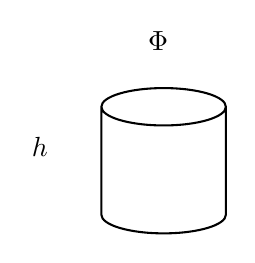
\begin{tikzpicture}[x=0.75pt,y=0.75pt,yscale=-1,xscale=1]
%uncomment if require: \path (0,412); %set diagram left start at 0, and has height of 412

%Shape: Can [id:dp9082674567153455] 
\draw   (411,215) -- (411,267) .. controls (411,271.97) and (397.57,276) .. (381,276) .. controls (364.43,276) and (351,271.97) .. (351,267) -- (351,215) .. controls (351,210.03) and (364.43,206) .. (381,206) .. controls (397.57,206) and (411,210.03) .. (411,215) .. controls (411,219.97) and (397.57,224) .. (381,224) .. controls (364.43,224) and (351,219.97) .. (351,215) ;

% Text Node
\draw (372,177.4) node [anchor=north west][inner sep=0.75pt]    {$\Phi $};
% Text Node
\draw (316,228.4) node [anchor=north west][inner sep=0.75pt]    {$h$};


\end{tikzpicture}


$V_{\text{цилиндра}} = h \cdot S(\Phi)$



\tikzset{every picture/.style={line width=0.75pt}} %set default line width to 0.75pt        

\begin{tikzpicture}[x=0.75pt,y=0.75pt,yscale=-1,xscale=1]
%uncomment if require: \path (0,412); %set diagram left start at 0, and has height of 412

%Shape: Polygon Curved [id:ds4295767736169027] 
\draw   (225,196) .. controls (245,186) and (335,176) .. (315,196) .. controls (295,216) and (295,226) .. (315,256) .. controls (335,286) and (245,286) .. (225,256) .. controls (205,226) and (205,206) .. (225,196) -- cycle ;
%Straight Lines [id:da544386965370033] 
\draw    (137,313) -- (407,313) ;
%Straight Lines [id:da5158515259785943] 
\draw  [dash pattern={on 0.84pt off 2.51pt}]  (209,126) -- (209,314) ;
%Straight Lines [id:da06882816394815783] 
\draw  [dash pattern={on 0.84pt off 2.51pt}]  (237,126) -- (237,314) ;
%Straight Lines [id:da915255431427515] 
\draw  [dash pattern={on 0.84pt off 2.51pt}]  (268,130) -- (268,318) ;
%Straight Lines [id:da5220043005403088] 
\draw  [dash pattern={on 0.84pt off 2.51pt}]  (293,125) -- (293,313) ;
%Straight Lines [id:da807165342443387] 
\draw  [dash pattern={on 0.84pt off 2.51pt}]  (317,125) -- (317,313) ;

% Text Node
\draw (203,327.4) node [anchor=north west][inner sep=0.75pt]    {$a$};
% Text Node
\draw (317,329.4) node [anchor=north west][inner sep=0.75pt]    {$b$};
% Text Node
\draw (199,353.4) node [anchor=north west][inner sep=0.75pt]    {$x_{0}$};
% Text Node
\draw (315,351.4) node [anchor=north west][inner sep=0.75pt]    {$x_{n}$};
% Text Node
\draw (231,353.4) node [anchor=north west][inner sep=0.75pt]    {$x_{1}$};


\end{tikzpicture}

"блинчик" $ = \{ (x, y, z) | x \in [x_{j - 1}, x_j], (y, z) \in T(x)\}$ --- почти цилиндр

Если предположить, что $\forall \delta \subset [a, b] $ среди сечений соотв. $x \in \delta$ есть наибольшее и наименьшее по включению, то формулу доказать можно.

$x_*(\delta), x^*(\delta)$ --- абсцисы минимального и максимального сечений. $ \hence$ $(x_j - x_{j - 1}) \cdot S(T(x_ *[x_{j - 1}, x_j])) \leqslant V(\text{блинчика}) \leqslant (x_j - x_{j - 1}) \cdot S(T(x^*[x_{j - 1}, x_j]))$. Складываем и получаем интегральную сумму. 

$\but$ это работает в очень специфических ситуациях. Зато для тел вращения все хорошо.

$T = \{ (x, y, z) | \sqrt(y ^ 2 + z ^ 2) \leqslant f(x) \}, f \in C[a, b], f \geqslant 0$




\tikzset{every picture/.style={line width=0.75pt}} %set default line width to 0.75pt        

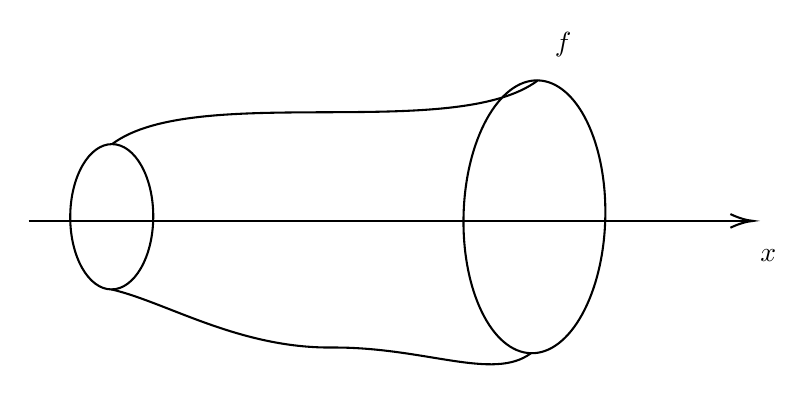
\begin{tikzpicture}[x=0.75pt,y=0.75pt,yscale=-1,xscale=1]
%uncomment if require: \path (0,412); %set diagram left start at 0, and has height of 412

%Straight Lines [id:da21011944043749586] 
\draw    (112,266) -- (459,266) ;
\draw [shift={(461,266)}, rotate = 180] [color={rgb, 255:red, 0; green, 0; blue, 0 }  ][line width=0.75]    (10.93,-3.29) .. controls (6.95,-1.4) and (3.31,-0.3) .. (0,0) .. controls (3.31,0.3) and (6.95,1.4) .. (10.93,3.29)   ;
%Shape: Ellipse [id:dp20031252116655374] 
\draw   (152.16,229) .. controls (163.2,229.05) and (172.09,244.76) .. (172,264.09) .. controls (171.91,283.42) and (162.89,299.05) .. (151.84,299) .. controls (140.8,298.95) and (131.91,283.24) .. (132,263.91) .. controls (132.09,244.58) and (141.11,228.95) .. (152.16,229) -- cycle ;
%Shape: Ellipse [id:dp983084836390024] 
\draw   (357.32,198.29) .. controls (376.18,198.77) and (390.71,228.58) .. (389.78,264.89) .. controls (388.86,301.19) and (372.83,330.23) .. (353.97,329.74) .. controls (335.12,329.26) and (320.59,299.45) .. (321.51,263.15) .. controls (322.44,226.84) and (338.47,197.8) .. (357.32,198.29) -- cycle ;
%Curve Lines [id:da08324117723612168] 
\draw    (152.16,229) .. controls (192.16,199) and (317.32,228.29) .. (357.32,198.29) ;
%Curve Lines [id:da4526472779035364] 
\draw    (151.84,299) .. controls (178,305) and (213.05,327.34) .. (258,327) .. controls (302.95,326.66) and (335.84,343.34) .. (353.97,329.74) ;

% Text Node
\draw (463,278.4) node [anchor=north west][inner sep=0.75pt]    {$x$};
% Text Node
\draw (364,173.4) node [anchor=north west][inner sep=0.75pt]    {$f$};


\end{tikzpicture}

$V(T) = \int_a^b \pi f^2(x) dx$


\quad

Как найти площадь поверхности?



\tikzset{every picture/.style={line width=0.75pt}} %set default line width to 0.75pt        

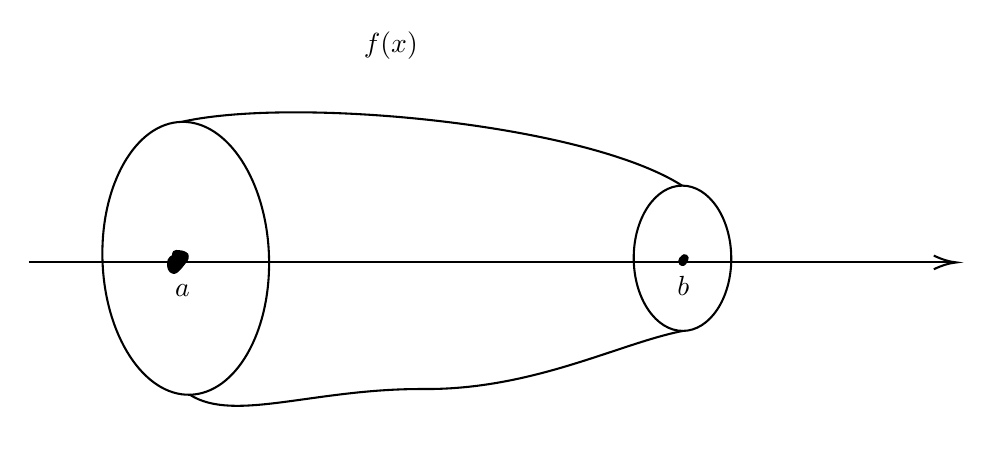
\begin{tikzpicture}[x=0.75pt,y=0.75pt,yscale=-1,xscale=1]
%uncomment if require: \path (0,412); %set diagram left start at 0, and has height of 412

%Straight Lines [id:da21011944043749586] 
\draw    (41,266) -- (486,266) ;
\draw [shift={(488,266)}, rotate = 180] [color={rgb, 255:red, 0; green, 0; blue, 0 }  ][line width=0.75]    (10.93,-3.29) .. controls (6.95,-1.4) and (3.31,-0.3) .. (0,0) .. controls (3.31,0.3) and (6.95,1.4) .. (10.93,3.29)   ;
%Shape: Ellipse [id:dp20031252116655374] 
\draw   (355.81,229) .. controls (342.83,229.05) and (332.39,244.76) .. (332.49,264.09) .. controls (332.59,283.42) and (343.19,299.05) .. (356.17,299) .. controls (369.15,298.95) and (379.59,283.24) .. (379.49,263.91) .. controls (379.39,244.58) and (368.79,228.95) .. (355.81,229) -- cycle ;
%Shape: Ellipse [id:dp983084836390024] 
\draw   (114.69,198.28) .. controls (92.54,198.76) and (75.46,228.58) .. (76.54,264.88) .. controls (77.63,301.19) and (96.46,330.23) .. (118.62,329.75) .. controls (140.77,329.27) and (157.85,299.45) .. (156.77,263.15) .. controls (155.68,226.84) and (136.85,197.8) .. (114.69,198.28) -- cycle ;
%Curve Lines [id:da08324117723612168] 
\draw    (355.81,229) .. controls (308.8,199) and (169,186) .. (114.69,198.28) ;
%Curve Lines [id:da4526472779035364] 
\draw    (356.18,299) .. controls (325.43,305) and (284.24,327.34) .. (231.42,327) .. controls (178.59,326.66) and (139.93,343.34) .. (118.62,329.74) ;
%Shape: Free Drawing [id:dp06649896024913649] 
\draw  [color={rgb, 255:red, 0; green, 0; blue, 0 }  ,draw opacity=1 ][line width=3] [line join = round][line cap = round] (112,262) .. controls (112.48,262) and (117.6,262.08) .. (116,264) .. controls (114.33,266) and (110.63,271.53) .. (110,269) .. controls (109.02,265.09) and (109.83,264) .. (113,264) ;
%Shape: Free Drawing [id:dp33007852384515557] 
\draw  [color={rgb, 255:red, 0; green, 0; blue, 0 }  ,draw opacity=1 ][line width=3] [line join = round][line cap = round] (357,264) .. controls (356.05,264.95) and (356,266.83) .. (356,265) ;

% Text Node
\draw (110,275.4) node [anchor=north west][inner sep=0.75pt]    {$a$};
% Text Node
\draw (352,271.4) node [anchor=north west][inner sep=0.75pt]    {$b$};
% Text Node
\draw (201,153.4) node [anchor=north west][inner sep=0.75pt]    {$f( x)$};


\end{tikzpicture}

$S_{\text{пов}} = \int_a^b 2\pi f$  --- неверная формула

$S_{\text{пов}} = \int_a^b 2\pi f \sqrt{1 + (f')^2}$  --- верная формула

\example (Интеграл Пуассона) $\int_{-\infty}^{+\infty} e ^ {-x^2} dx = I$



\tikzset{every picture/.style={line width=0.75pt}} %set default line width to 0.75pt        

\begin{tikzpicture}[x=0.75pt,y=0.75pt,yscale=-1,xscale=1]
%uncomment if require: \path (0,412); %set diagram left start at 0, and has height of 412

%Shape: Axis 2D [id:dp7224301703480168] 
\draw  (91,282.24) -- (504,282.24)(292.74,134) -- (292.74,358) (497,277.24) -- (504,282.24) -- (497,287.24) (287.74,141) -- (292.74,134) -- (297.74,141)  ;
%Curve Lines [id:da38662910461432465] 
\draw    (90,278) .. controls (135,286) and (259,253) .. (291,255) .. controls (323,257) and (454,284) .. (488,278) ;

% Text Node
\draw (333,224.4) node [anchor=north west][inner sep=0.75pt]    {$y\ =\ e^{-x^{2}}$};


\end{tikzpicture}


Вращаем отн. оси y


Сечем по y



\tikzset{every picture/.style={line width=0.75pt}} %set default line width to 0.75pt        

\begin{tikzpicture}[x=0.75pt,y=0.75pt,yscale=-1,xscale=1]
%uncomment if require: \path (0,412); %set diagram left start at 0, and has height of 412

%Shape: Axis 2D [id:dp7224301703480168] 
\draw  (91,282.24) -- (504,282.24)(292.74,134) -- (292.74,358) (497,277.24) -- (504,282.24) -- (497,287.24) (287.74,141) -- (292.74,134) -- (297.74,141)  ;
%Curve Lines [id:da38662910461432465] 
\draw    (90,278) .. controls (135,286) and (259,253) .. (291,255) .. controls (323,257) and (454,284) .. (488,278) ;
%Straight Lines [id:da9343639811351652] 
\draw  [dash pattern={on 0.84pt off 2.51pt}]  (228,265) -- (349,265) ;
%Straight Lines [id:da8088627525116787] 
\draw  [dash pattern={on 0.84pt off 2.51pt}]  (171,273) -- (405,273) ;

% Text Node
\draw (333,224.4) node [anchor=north west][inner sep=0.75pt]    {$y\ =\ e^{-x^{2}}$};
% Text Node
\draw (272,291.4) node [anchor=north west][inner sep=0.75pt]    {$0$};
% Text Node
\draw (277,229.4) node [anchor=north west][inner sep=0.75pt]    {$1$};


\end{tikzpicture}

$\pi \int_0^1 (\sqrt(-\log y)) ^ 2 dy = \pi \int_0^1 -\log y dy = \pi (y - y \log y ) \bigg | _0^1 = \pi$
 

Теперь нарежем параллельно оси y


Тогда сечение будет иметь вид
$0 \leqslant y \leqslant e ^ {-(x ^ 2 + z ^ 2)}$

$T(a) = \{ (y, z) : 0 \leqslant y \leqslant e^{-(x ^ 2 + z ^ 2)}\}$

$S(T(a)) = \int_{-infty}^{\infty} e ^ {-a ^ 2 + z ^ 2} dz = e ^ {-a ^ 2} I$

$V = \int_{-\infty}^{+\infty} S(T(x)) dx = I \int_{-\infty}^{+\infty} e ^ {- x ^ 2} dx = I ^ 2$

\end{enumerate}


\subsection{Длниы путей}




\tikzset{every picture/.style={line width=0.75pt}} %set default line width to 0.75pt        

\begin{tikzpicture}[x=0.75pt,y=0.75pt,yscale=-1,xscale=1]
%uncomment if require: \path (0,412); %set diagram left start at 0, and has height of 412

%Curve Lines [id:da2658951326576444] 
\draw    (208,238) .. controls (248,208) and (319,132) .. (351,189) ;

% Text Node
\draw (190,253.4) node [anchor=north west][inner sep=0.75pt]    {$t=a$};
% Text Node
\draw (359,196.4) node [anchor=north west][inner sep=0.75pt]    {$t=b$};
% Text Node
\draw (255,222.4) node [anchor=north west][inner sep=0.75pt]    {$( x( t) ,\ y( t))$};


\end{tikzpicture}


Подход физиков --- найти скорость : $\sqrt{x'(t) ^ 2 + y'(t) ^ 2}$ и взять интерграл $\int_a ^ b \sqrt{x'(t) ^ 2 + y'(t) ^ 2} dt$ --- длина кривой
